%% LyX 2.1.0dev created this file.  For more info, see http://www.lyx.org/.
%% Do not edit unless you really know what you are doing.
\documentclass[english,conference]{IEEEtran}
\usepackage[T1]{fontenc}
\usepackage[utf8]{luainputenc}
\usepackage{array}
\usepackage{multirow}
\usepackage{amsmath}
\usepackage{amssymb}
\usepackage{stmaryrd}
\usepackage{graphicx}
\usepackage{esint}

\makeatletter

%%%%%%%%%%%%%%%%%%%%%%%%%%%%%% LyX specific LaTeX commands.
%% Because html converters don't know tabularnewline
\providecommand{\tabularnewline}{\\}

%%%%%%%%%%%%%%%%%%%%%%%%%%%%%% User specified LaTeX commands.


% manually specify the path to it: e.g.,
% \documentclass[conference]{../sty/IEEEtran}

\usepackage{times}\usepackage{psfig}% Add all your packages here

% correct bad hyphenation here
\hyphenation{op-tical net-works semi-conduc-tor IEEEtran}

\IEEEoverridecommandlockouts    % to create the author's affliation portion
                % using \thanks

\textwidth 178mm    % <------ These are the adjustments we made 10/18/2005
\textheight 239mm   % You may or may not need to adjust these numbers again
\oddsidemargin -7mm
\evensidemargin -7mm
\topmargin -6mm
\columnsep 5mm

\makeatother

\usepackage{babel}
\begin{document}
% paper title: Must keep \ \\ \LARGE\bf in it to leave enough margin.



\title{\ \\
 \textbf{A Unified Approach to Fuzzy and Probabilistic Uncertain Interval
Algebra}}


\author{Keyvan Mir Mohammad Sadeghi and Ben Goertzel}

\maketitle
% make the title area

\begin{abstract}
A novel approach to uncertain temporal inference is presented. Allen's
Interval Algebra is extended to fuzzy time-intervals via representing
the latter as trapeziums with distinct beginning, middle and end.
An uncertain version of the Interval Algebra composition table is
developed via running a computer simulation in which a large number
of fuzzy time-intervals are drawn from an assumed probability distribution,
and using machine learning to induce uncertain compositional rules
that hold approximately across the corpus of simulated intervals. 
\end{abstract}
% no key words



\section{Introduction}

\PARstart{B}{en} can write a couple intro paragraphs \cite{PLN}


\subsection{\label{sub:Allen-Interval-Algebra}Allen Interval Algebra}

One way to approach temporal reasoning is to represent the events
in terms of \emph{intervals}. An interval captures some portion of
time within which some features hold, then a temporal event could
be represented as \textbf{\emph{{[}a, b{]}}} where \emph{a} is the
beginning time-step of the event and \emph{b} is the ending. There
has been many works focused on addressing interval handling for temporal
inference, most notable of these are Allen's Interval Algebra (IA)
\cite{Allen} and Interval Temporal Logic (ITL) \cite{Moszkowski-Thesis,Moszkowski-Paper}. 

The foundation that IA is built on in treating intervals is to set
aside the actual time frames in which events occur, and instead, work
with the \emph{relation} between two intervals. To this end, IA defines
thirteen basic relations that address three desired qualities:
\begin{description}
\item [{Distinct}] the set of 13 relations constitute a partitioning over
the relation space
\item [{Exhaustive}] any pair of intervals can only be described by only
one of the relations
\item [{Qualitative}] the ground for comparing two intervals is how they
relate, as opposed to the time frames they lay in (quantitative)
\end{description}
Each Allen relation poses four constraints, for two intervals to be
qualified as holding the relation, they should satisfy all four. For
instance, assuming two intervals \emph{a} and \emph{b} are given,
the relation \emph{\{s\}} (starts) is defined as $beginning_{a}=beginning_{b}$
AND $beginning_{a}<ending_{b}$ AND $ending_{a}>beginning_{b}$ AND
$ending_{a}<ending_{b}$. The set of thirteen Allen relations are
shown in Table \ref{tab:Temporal-Relations}.

Having the relations in place, IA continues with defining operations
on relations:
\begin{description}
\item [{Complement}] denoted as \emph{\textasciitilde{}r}, complement of
set \emph{r} is the set of all relations not present in \emph{r}
\item [{Converse}] or \emph{!r}, is the set of relations obtained from
substituting intervals \emph{a} and \emph{b} in the original relation
\emph{a\{r\}b}
\item [{Intersection}] shown by \emph{r\textasciicircum{}s} is the set
of relations present in both \emph{r} and \emph{s}
\item [{Union}] \emph{r+s}, set of relations present in either \emph{r}
or \emph{s}
\item [{Composition}] \emph{r.s}, the set of all possible relations between
intervals \emph{a} and \emph{c}, having \emph{a\{r\}b} and \emph{b\{s\}c}
\end{description}
Examples for these operations are presented in Table \ref{tab:Examples-of-operations},
Table \ref{tab:Composition} shows composition of \emph{a\{r\}b} and
\emph{b\{s\}c} for singular \emph{r} and \emph{s}.

\begin{table}
\protect\caption{\label{tab:Temporal-Relations}Temporal relations in Interval Algebra}


\centering{}%
\begin{tabular}{|c|c|c|}
\hline 
Precedes \emph{(p)} & Meets \emph{(m)} & Overlaps \emph{(o)}\tabularnewline
\hline 
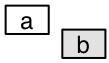
\includegraphics[scale=0.4]{p} & 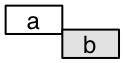
\includegraphics[scale=0.4]{m} & 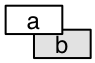
\includegraphics[scale=0.4]{o}\tabularnewline
\hline 
Preceded by \emph{(P)} & Met by \emph{(M)} & Overlapped by \emph{(O)}\tabularnewline
\hline 
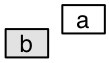
\includegraphics[scale=0.4]{pi} & 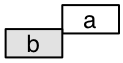
\includegraphics[scale=0.4]{mi} & 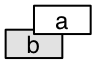
\includegraphics[scale=0.4]{oi}\tabularnewline
\hline 
Finished by \emph{(F)} & Contains \emph{(D)} & Starts \emph{(s)}\tabularnewline
\hline 
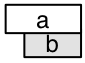
\includegraphics[scale=0.4]{fi} & 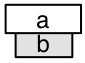
\includegraphics[scale=0.4]{di} & 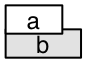
\includegraphics[scale=0.4]{s}\tabularnewline
\hline 
Finishes \emph{(f)} & During \emph{(d)} & Started by \emph{(S)}\tabularnewline
\hline 
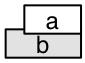
\includegraphics[scale=0.4]{f} & 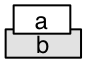
\includegraphics[scale=0.4]{d} & 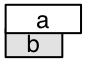
\includegraphics[scale=0.4]{si}\tabularnewline
\hline 
\multicolumn{3}{|c|}{Equals \emph{(e)}}\tabularnewline
\hline 
\multicolumn{3}{|c|}{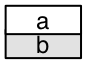
\includegraphics[scale=0.4]{e}}\tabularnewline
\hline 
\end{tabular}
\end{table}


\begin{table}
\protect\caption{\label{tab:Examples-of-operations}Examples of operations on relations}


\centering{}%
\begin{tabular}{|c|c|}
\hline 
\textbf{Complement} & \textbf{Converse}\tabularnewline
\hline 
\emph{\textasciitilde{}(p) = (moFDseSdfOMP)} & \emph{!(p) = (P)}\tabularnewline
\hline 
\emph{\textasciitilde{}(pmoFD) = (seSdfOMP)} & \emph{!(pmoFD) = (dfOMP)}\tabularnewline
\hline 
\multirow{2}{*}{\textasciitilde{}() = (pmoFDseSdfOMP)} & \emph{!(mM) = (mM)}\tabularnewline
\cline{2-2} 
 & \emph{!() = ()}\tabularnewline
\hline 
\textbf{Intersection} & \textbf{Union}\tabularnewline
\hline 
\emph{(pmo)\textasciicircum{}(FDseS) = ()} & \emph{(pmo)+(FDseS) = (pmoFDseS)}\tabularnewline
\hline 
\emph{(pFsSf)\textasciicircum{}(pmoFD) = (pF)} & \emph{(pFsSf)+(pmoFD) = (pmoFDsSf)}\tabularnewline
\hline 
\emph{(pmo)\textasciicircum{}(pmo) = (pmo)} & \emph{(pmo)+(pmo) = (pmo)}\tabularnewline
\hline 
\multicolumn{2}{|c|}{\textbf{Composition}}\tabularnewline
\hline 
\multicolumn{2}{|c|}{\emph{(m).(m) = (p)}}\tabularnewline
\hline 
\multicolumn{2}{|c|}{\emph{(pm).(pm) = (p)}}\tabularnewline
\hline 
\multicolumn{2}{|c|}{\emph{(oFD).(oFDseS) = (pmoFD)}}\tabularnewline
\hline 
\end{tabular}
\end{table}


\begin{table}
\protect\caption{\label{tab:Composition}Composition in Interval Algebra}


\begin{tabular}{|c|c|c|c|c|c|c|c|c|c|c|c|c|c|}
\hline 
 & \textbf{p} & \textbf{m} & \textbf{o} & \textbf{F} & \textbf{D} & \textbf{s} & \textbf{e} & \textbf{S} & \textbf{d} & \textbf{f} & \textbf{O} & \textbf{M} & \textbf{P}\tabularnewline
\hline 
\textbf{p} & \emph{(p)} & \emph{(p)} & \emph{(p)} & \emph{(p)} & \emph{(p)} & \emph{(p)} & \emph{(p)} & \emph{(p)} & \emph{(pmosd)} & \emph{(pmosd)} & \emph{(pmosd)} & \emph{(pmosd)} & \emph{full}\tabularnewline
\hline 
\textbf{m} & \emph{(p)} & \emph{(p)} & \emph{(p)} & \emph{(p)} & \emph{(p)} & \emph{(m)} & \emph{(m)} & \emph{(m)} & \emph{(osd)} & \emph{(osd)} & \emph{(osd)} & \emph{(Fef)} & \emph{(DSOMP)}\tabularnewline
\hline 
\textbf{o} & \emph{(p)} & \emph{(p)} & \emph{(pmo)} & \emph{(pmo)} & \emph{(pmoFD)} & \emph{(o)} & \emph{(o)} & \emph{(oFD)} & \emph{(osd)} & \emph{(osd)} & \emph{concur} & \emph{(DSO)} & \emph{(DSOMP)}\tabularnewline
\hline 
\textbf{F} & \emph{(p)} & \emph{(m)} & \emph{(o)} & \emph{(F)} & \emph{(D)} & \emph{(o)} & \emph{(F)} & \emph{(D)} & \emph{(osd)} & \emph{(Fef)} & \emph{(DSO)} & \emph{(DSO)} & \emph{(DSOMP)}\tabularnewline
\hline 
\textbf{D} & \emph{(pmoFD)} & \emph{(oFD)} & \emph{(oFD)} & \emph{(D)} & \emph{(D)} & \emph{(oFD)} & \emph{(D)} & \emph{(D)} & \emph{concur} & \emph{(DSO)} & \emph{(DSO)} & \emph{(DSO)} & \emph{(DSOMP)}\tabularnewline
\hline 
\textbf{s} & \emph{(p)} & \emph{(p)} & \emph{(pmo)} & \emph{(pmo)} & \emph{(pmoFD)} & \emph{(s)} & \emph{(s)} & \emph{(seS)} & \emph{(d)} & \emph{(d)} & \emph{(dfO)} & \emph{(M)} & \emph{(P)}\tabularnewline
\hline 
\textbf{e} & \emph{(p)} & \emph{(m)} & \emph{(o)} & \emph{(F)} & \emph{(D)} & \emph{(s)} & \emph{(e)} & \emph{(S)} & \emph{(d)} & \emph{(f)} & \emph{(O)} & \emph{(M)} & \emph{(P)}\tabularnewline
\hline 
\textbf{S} & \emph{(pmoFD)} & \emph{(oFD)} & \emph{(oFD)} & \emph{(D)} & \emph{(D)} & \emph{(seS)} & \emph{(S)} & \emph{(S)} & \emph{(dfO)} & \emph{(O)} & \emph{(O)} & \emph{(M)} & \emph{(P)}\tabularnewline
\hline 
\textbf{d} & \emph{(p)} & \emph{(p)} & \emph{(pmosd)} & \emph{(pmosd)} & \emph{full} & \emph{(d)} & \emph{(d)} & \emph{(dfOMP)} & \emph{(d)} & \emph{(d)} & \emph{(dfOMP)} & \emph{(P)} & \emph{(P)}\tabularnewline
\hline 
\textbf{f} & \emph{(p)} & \emph{(m)} & \emph{(osd)} & \emph{(Fef)} & \emph{(DSOMP)} & \emph{(d)} & \emph{(f)} & \emph{(OMP)} & \emph{(d)} & \emph{(f)} & \emph{(OMP)} & \emph{(P)} & \emph{(P)}\tabularnewline
\hline 
\textbf{O} & \emph{(pmoFD)} & \emph{(oFD)} & \emph{concur} & \emph{(DSO)} & \emph{(DSOMP)} & \emph{(dfO)} & \emph{(O)} & \emph{(OMP)} & \emph{(dfO)} & \emph{(O)} & \emph{(OMP)} & \emph{(P)} & \emph{(P)}\tabularnewline
\hline 
\textbf{M} & \emph{(pmoFD)} & \emph{(seS)} & \emph{(dfO)} & \emph{(M)} & \emph{(P)} & \emph{(dfO)} & \emph{(M)} & \emph{(P)} & \emph{(dfO)} & \emph{(M)} & \emph{(P)} & \emph{(P)} & \emph{(P)}\tabularnewline
\hline 
\textbf{P} & \emph{full} & \emph{(dfOMP)} & \emph{(dfOMP)} & \emph{(P)} & \emph{(P)} & \emph{(dfOMP)} & \emph{(P)} & \emph{(P)} & \emph{(dfOMP)} & \emph{(P)} & \emph{(P)} & \emph{(P)} & \emph{(P)}\tabularnewline
\hline 
\end{tabular}
\end{table}



\subsection{\label{sub:Fuzzy-Interval-Algebra}Fuzzy Interval Algebra}

The original IA provides sufficient means for crisp reasoning. Moreover,
one can use the classic IA for systems that have their knowledge represented
as \emph{TRUE} and \emph{FALSE} propositions. However, most modern
inference engines utilise some sort of fuzzy/probabilistic representation
instead of (or in parallel to) the old-fashioned binary ones. Therefore,
such systems will not be able to use IA in it's basic form. Accordingly,
a substantial amount of work has been carried out to adapt IA to the
aforementioned paradigms. Related works that have been done in this
regards fall into two general categories: I) Probabilistic extensions
and II) Fuzzy models of IA. Each of these approaches are designed
to solve a different set of problems/setups.

Probabilistic models are usually adopted in scenarios where there
is some level of uncertainty involved in reasoning about given pieces
of knowledge. The probabilistic methods themselves are scattered in
many different sub-paradigms. So in order to offer a generalised solution
that could be adopted by all systems in which some probabilistic representations
is used, it is often the case that probabilistic extensions of IA
expand on the concept of \textquotedbl{}probability distributions\textquotedbl{}.

Keyvan should briefly explain why we didn't just use their work


\section{A Generic Fuzzy/Probabilistic Model of Interval Algebra}

As described in Section \ref{sub:Fuzzy-Interval-Algebra}, the previous
models of IA fail to provide a mapping between the fuzzy and probabilistic
paradigms. The main focus here, accordingly, is to formalise a minimal
framework that supports both approaches. A minimum ground for such
framework, therefore, is constituted from the following features:
\begin{description}
\item [{Accommodate~the~Fuzzy~Model}] one should be able to encode intervals
in terms of fuzzy sets, and also be able to query the degree to which
the event is happening in any interval. Let us call this \textbf{\emph{(ACC-FUZZ)}}
\item [{Accommodate~the~Probabilistic~Model}] it should be possible
to define the interval in terms of probability distributions \textbf{\emph{(ACC-PROB)}}
\item [{Reduction~to~original~IA}] the model must be reducible to the
original IA, i.e. the necessary means for defining a crisp interval
and the IA operations both should be present, and the logic of interval
relations should be analogous to that of Allen's \textbf{\emph{(REDC-IA)}}
\item [{Extensibility}] the framework should allow customisation of the
logic behind relation handling \textbf{\emph{(EXTN)}}
\end{description}
First off, the unit of work will be changed to \emph{event} from \emph{interval}.
The reason for the name change is that an Allen \emph{interval} is
a one dimensional entity whereas an \emph{event} has two dimensions,
time and certainty. Starting with \emph{ACC-PROB}, an event is described
by two probability distributions, \emph{dist\_beg} and \emph{dist\_end}.
\emph{dist\_beg} denotes the ``probability that event is in it's
beginning stage'', expanding on the original IA where beginning was
a single point, a probabilistic beginning would be a probability distribution
over the interval of \emph{{[}a, beginning{]}}. Similarly, \emph{dist\_end}
is the ``probability that event is in it's ending stage'', over
the \emph{{[}ending, b{]}} interval. For the event to be valid, \emph{dist\_beg}
and \emph{dist\_end} should satisfy the condition below:

\begin{center}
$\mu_{dist\textunderscore beg}<\text{\ensuremath{\mu}}_{dist\textunderscore end}$
\par\end{center}

\begin{center}
read: mean of \emph{dist\_beg} should be lower than mean of \emph{dist\_end}
\par\end{center}

We then define a $membership\textunderscore function$ so as to address
\emph{ACC-FUZZ}:

\begin{center}
$membership\textunderscore function\left(t\right)=dist\textunderscore beg.cdf\left(t\right)-dist\textunderscore end.cdf\left(t\right)$
\par\end{center}

\begin{center}
-- where \emph{cdf} is the cumulative distribution function of the
probability distribution
\par\end{center}

To query the fuzzy degree of the event in an interval, one should
use the \emph{Degree function}:

\begin{center}
$\text{\ensuremath{\mathcal{D}}}\left(mf\left(t\right),~\left[a,~b\right]\right)=\frac{\intop_{a}^{b}mf\left(t\right)dt}{b-a}$
\par\end{center}

\begin{center}
-- where \emph{mf} is the \emph{membership\_function} of the event
\par\end{center}

An event resulting from a normal and an exponential distribution is
shown in Fig \ref{fig:Event-Example}.

\begin{figure}
\begin{centering}
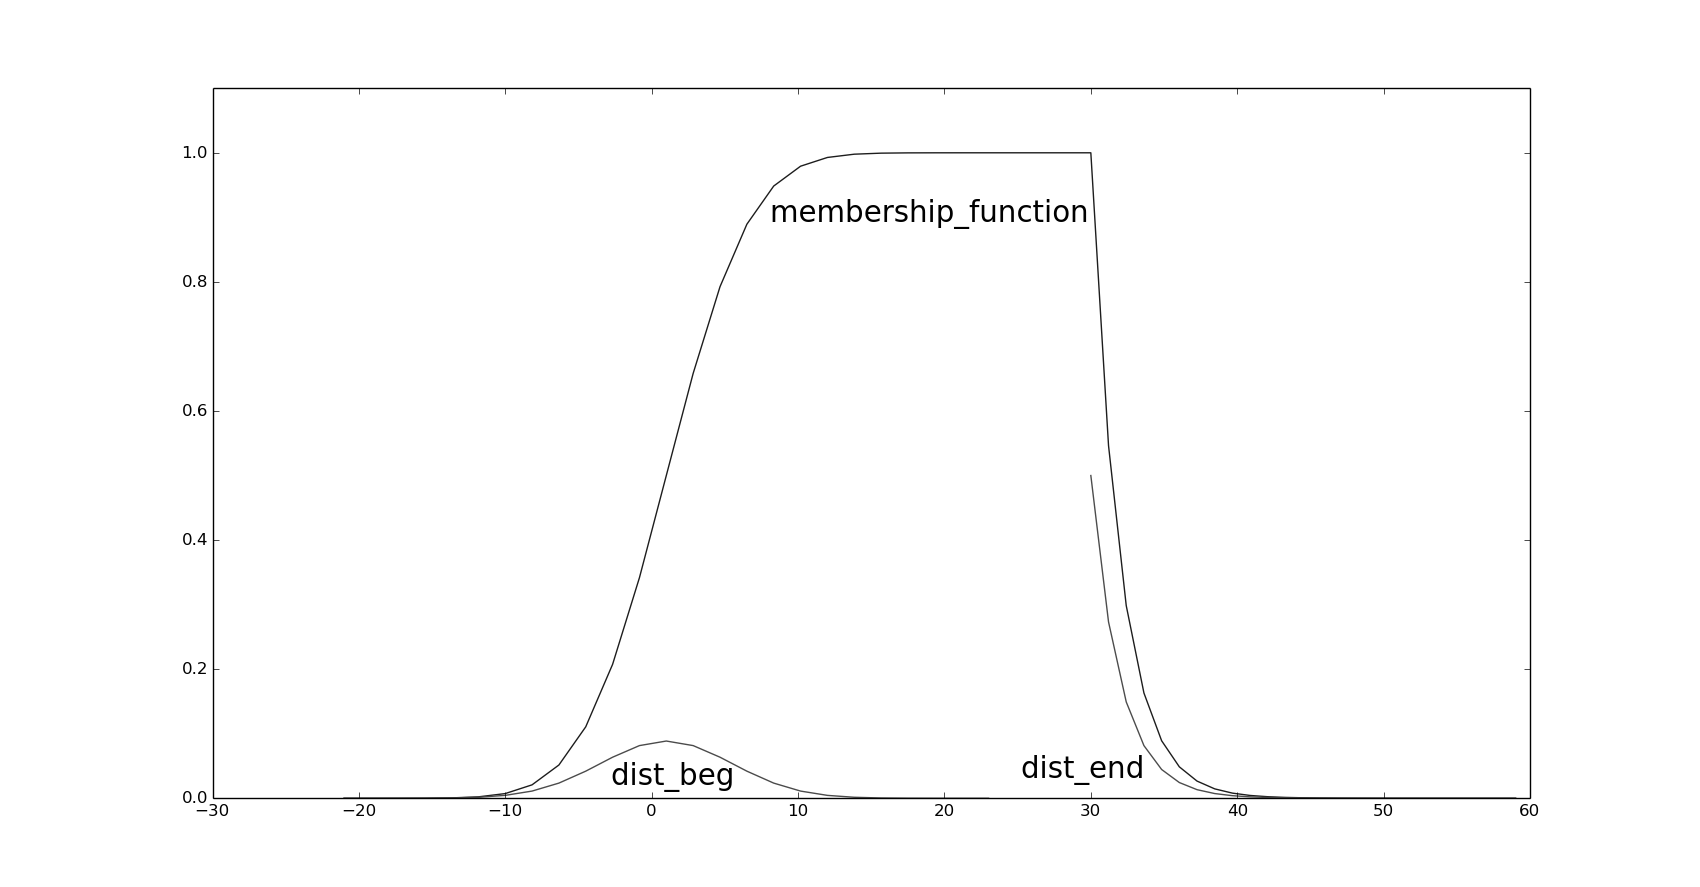
\includegraphics[scale=0.2]{Fig1}
\par\end{centering}

\protect\caption{\label{fig:Event-Example}Example of a temporal event}
\end{figure}


In the case that one would like to initialise an event by providing
fuzzy sets representing the \emph{membership\_function}, two sets
are required: one corresponding to the beginning portion of the event
and one for the ending. For the beginning set to be valid, it should
start with a value less than one in it's first time-step and climbs
up to one in the later steps. The ending set should start from one
and decrease over time. In addition, the first time-step of the beginning
set should have a lower value than the first one in the ending set.
Upon satisfaction of these conditions, one can constitute the corresponding
probability distributions, the beginning and ending sets could be
viewed as the \emph{cdf} functions of the distributions ($1-cdf$
in the case of the ending set), and the relating probability density
function (\emph{pdf}) would be the derivative of the \emph{cdf}. The
mean of such distribution is calculated by weighted averaging over
it's \emph{pdf} function (mean is usually used in calculating event
relations, therefore it is a requirement for any custom probability
distribution). This process is demonstrated in Fig \ref{fig:Fuzzy-Sets},
as evident in Fig \ref{fig:Fuzzy-Sets}b, the two sets can overlap
in which case the \emph{membership\_function} will not reach the value
one.

\begin{figure}
\begin{centering}
\begin{tabular}{c}
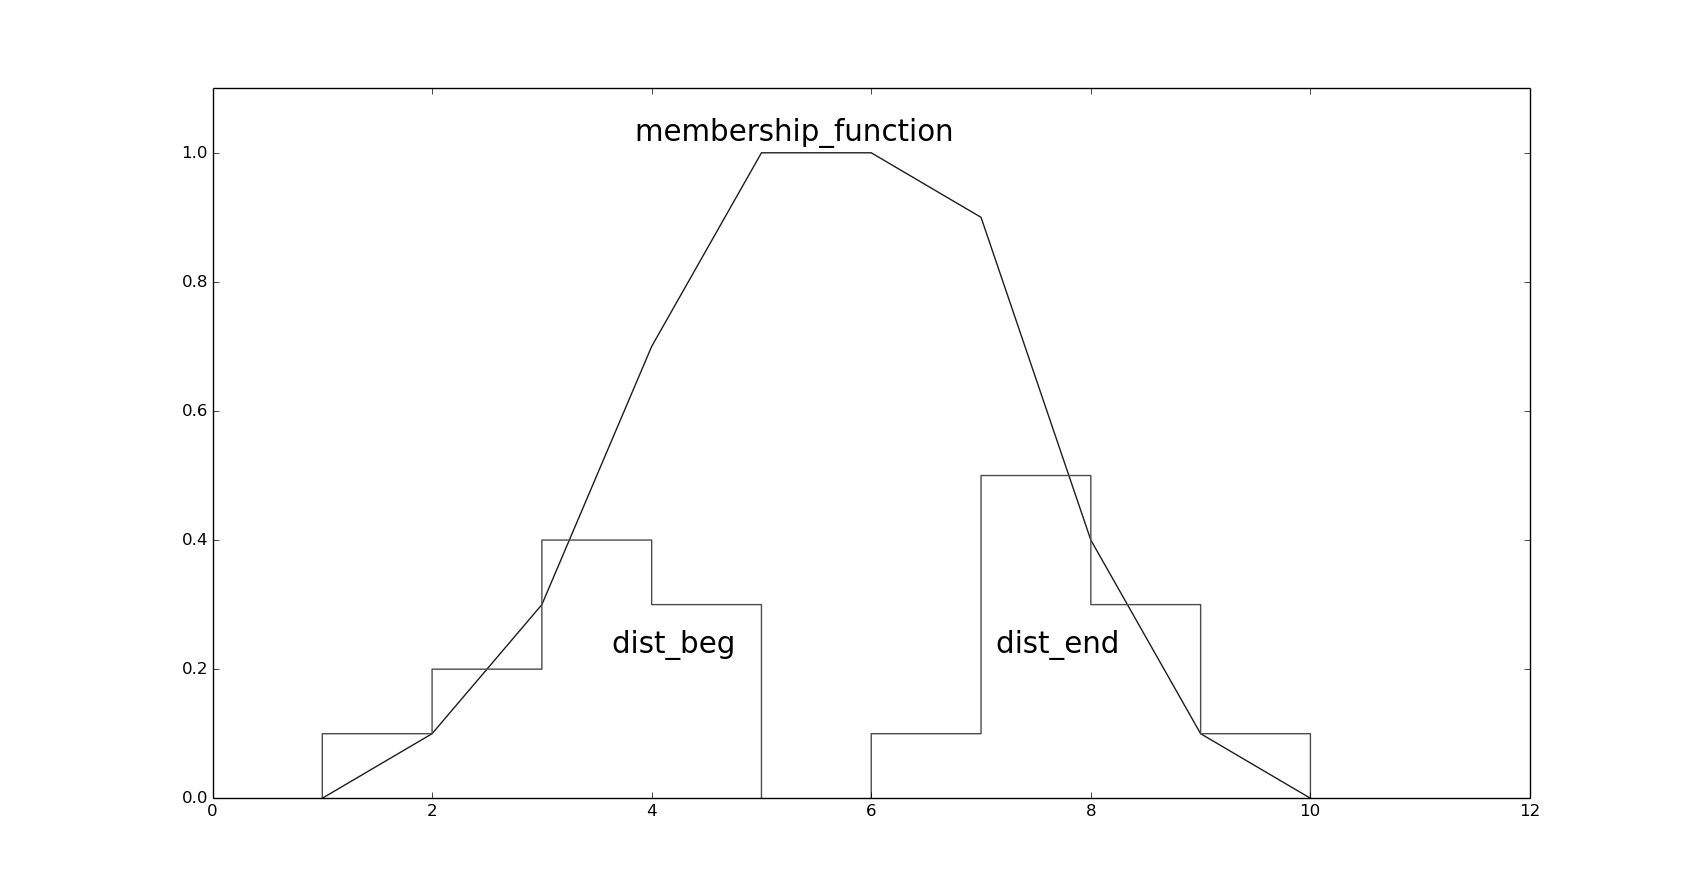
\includegraphics[scale=0.2]{Fig3a}\tabularnewline
\emph{a) set\_beg = \{1: 0, 2: 0.1, 3: 0.3, 4: 0.7, 5: 1\}, }\tabularnewline
\emph{set\_end = \{6: 1, 7: 0.9, 8: 0.6, 9: 0.1, 10: 0\}}\tabularnewline
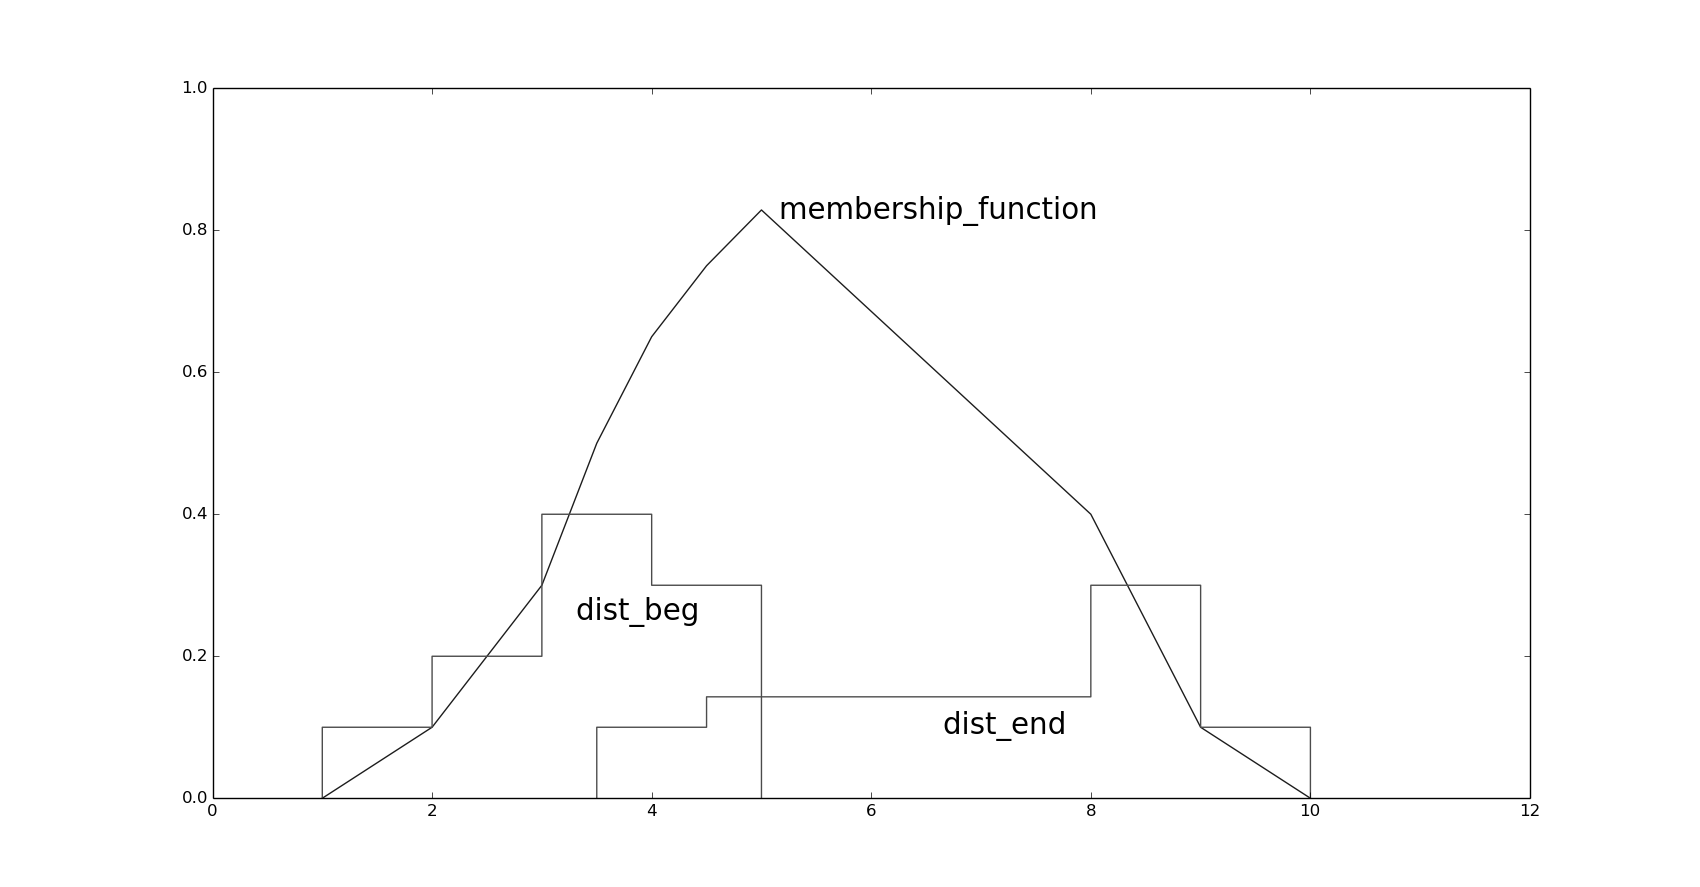
\includegraphics[scale=0.2]{Fig3b}\tabularnewline
\emph{a) set\_beg = \{1: 0, 2: 0.1, 3: 0.3, 4: 0.7, 5: 1\},}\tabularnewline
\emph{ set\_end = \{3.5: 1, 4.5: 0.9, 8: 0.6, 9: 0.1, 10: 0\}}\tabularnewline
\end{tabular}
\par\end{centering}

\protect\caption{\label{fig:Fuzzy-Sets}Mapping fuzzy sets to probability distributions}
\end{figure}


To be consistent with \emph{REDC-IA}, a custom distribution, \emph{point\_dist},
is defined as follows:

\begin{center}
$point\textunderscore dist\left(t\right)=uniform\left(t-\varepsilon,~t+\varepsilon\right),~\varepsilon\rightarrow\infty$
\par\end{center}

\emph{point\_dist} allows one to create crisp intervals, this is demonstrated
in Fig \ref{fig:Point-Dist}. Another requirement for \emph{REDC-IA}
is to handle interval relations in a manner that is analogous to the
original IA. Three functions are defined to do so:

\begin{center}
\emph{before(dist\_1, dist\_2), same(dist\_1, dist\_2) and after(dist\_1,
dist\_2)}
\par\end{center}

Having an implementation of the above functions at hand, one can calculate
degrees for each of the thirteen Allen relations. Taking the \emph{\{s\}}
(starts) relation example from Section \ref{sub:Allen-Interval-Algebra},
the degree for \emph{a\{s\}b} is calculated as:

\begin{center}
$same\left(dist\textunderscore beg_{a},~dist\textunderscore beg_{b}\right)\times before\left(dist\textunderscore beg_{a},~dist\textunderscore end_{b}\right)\times after\left(dist\textunderscore end_{a},~dist\textunderscore beg_{b}\right)\times before\left(dist\textunderscore end_{a},~dist\textunderscore end_{b}\right)$
\par\end{center}

Table \ref{tab:Operation-Mapping} shows the mapping from crisp interval
relations to distributional event relations. One can calculate degree
values for all of the IA relations in a manner similar to the above
example. These degree values can represent fuzzy degrees or probability
values according to their corresponding implementation, the only requirement
is that they be within \emph{{[}0, 1{]}}. The original IA operations
then can be mapped as follows:
\begin{description}
\item [{Complement}] \emph{\textasciitilde{}r} is calculated as $1-R$
for each \emph{$R\in r$}
\item [{Converse}] \emph{!r} is obtained by substituting \emph{a} and \emph{b}
in the relation's formula (which is defined in terms of \emph{before},
\emph{same} and \emph{after} this time around)
\item [{Intersection}] \emph{r\textasciicircum{}s} is calculated as $min\left(R,~S\right)$
for each $R=S,~R\in r~and~S\in s$
\item [{Union}] \emph{r+s} is calculated as $max\left(R,~S\right)$ for
each $R=S,~R\in r~and~S\in s$
\item [{Composition}] \emph{r.s} contains members based on the original
IA composition table, but since relations are not \emph{TRUE} and
\emph{FALSE} anymore, there should be a mapping mechanism. Section
\ref{sec:Composition} expands more on the composition problem.
\end{description}
The fact that one can adopt a custom version of of \emph{before},
\emph{same} and \emph{after} shows that the \emph{EXTN} requirement
is satisfied. Any implementation should qualify in the context of
the three original IA relation criteria, it should be \emph{Distinct}
in that the method partitions the relation space into \emph{before},
\emph{same}, and \emph{after}, \emph{Exhaustive} so that it calculates
a single value for each pair of distributions and naturally \emph{Quantitative}
as it calculates a value for the relation between the two distributions,
regardless of their time-frames, but according to their relation (e.g.
geometric). Sections \ref{sub:Convolution} and \ref{sub:Geometric-Mean}
went on to describe two different implementations of \emph{before},
\emph{same} and \emph{after}.

\begin{figure}
\begin{centering}
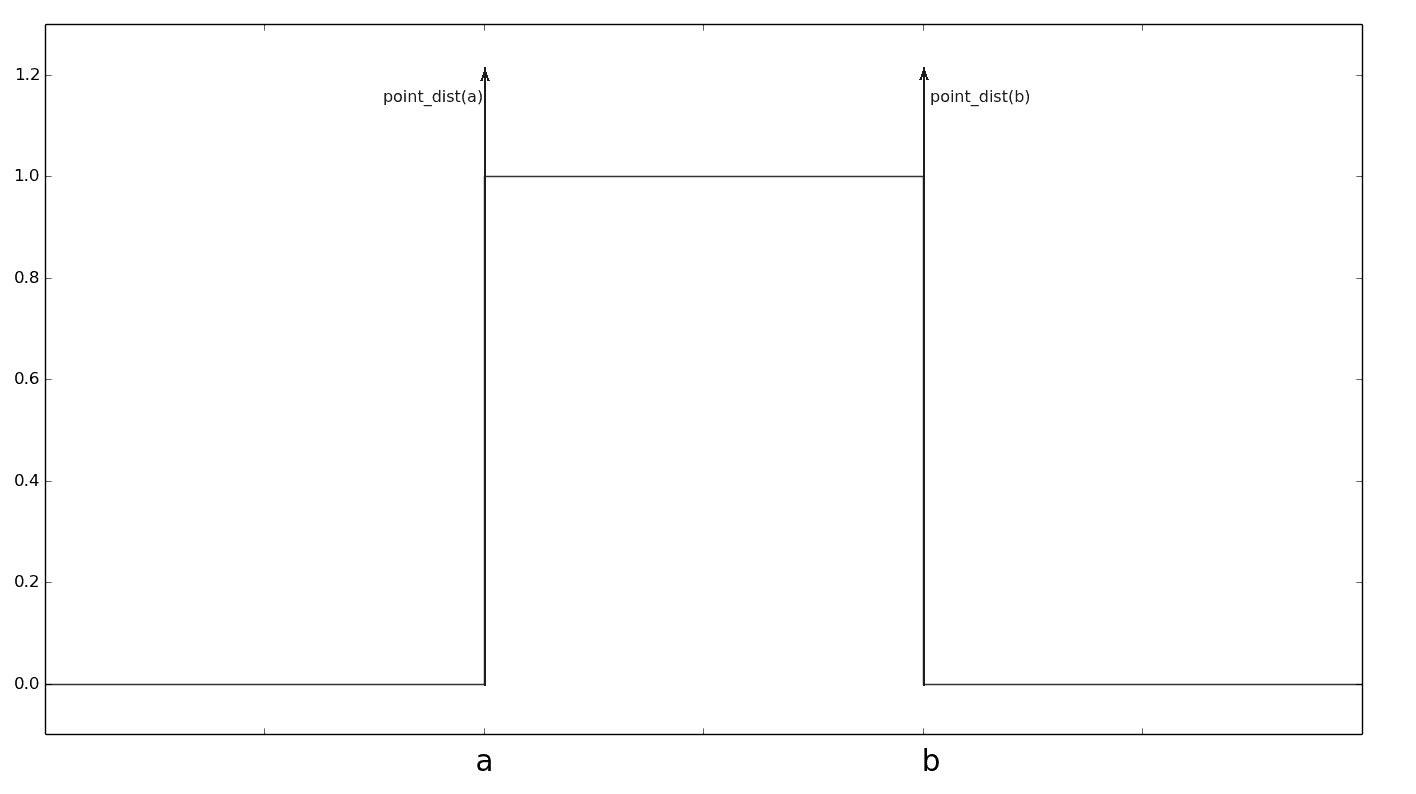
\includegraphics[scale=0.2]{Fig2}
\par\end{centering}

\protect\caption{\label{fig:Point-Dist}A crisp interval produced by \emph{point\_dist}}
\end{figure}


\begin{table}
\protect\caption{\label{tab:Operation-Mapping}Crisp interval to Distributional event
operation mapping}


\centering{}%
\begin{tabular}{|c|c|}
\hline 
\textbf{Crisp} & \textbf{Distributional}\tabularnewline
\hline 
\emph{point\_1 = point\_2} & \emph{same(dist\_1, dist\_2)}\tabularnewline
\hline 
\emph{point\_1 < point\_2} & \emph{before(dist\_1, dist\_2)}\tabularnewline
\hline 
\emph{point\_1 > point\_2} & \emph{after(dist\_1, dist\_2)}\tabularnewline
\hline 
\end{tabular}
\end{table}



\subsection{A Trapezium Model of Fuzzy/Probabilistic Intervals}

Now that the temporal events are defined in their broad form, it gets
to the point of proposing a specific instance that is suitable for
general problems. In doing so, it should be taken into account that
such generalisation must be capable of handling both uncertainty types,
direct and indirect (described in Section \ref{sub:Fuzzy-Interval-Algebra}).
In the case of indirect observation, it is a common practice to assume
a uniform uncertainty over the period of the beginning and ending
intervals, as in {[}1234{]}. Direct observation on the other hand
often involves knowledge coming from natural or artificial sources,
most of such events have either normal or exponential nature to them.
Interestingly, this has not been considered in related works in this
area such as {[}1234{]} and instead a uniform distribution of uncertainty
has been assumed. However, it is understandable why this path has
been taken, uniform distribution has the quality of being a meaningful
average over the set of different possible distributions. Accordingly,
the ``Trapezium Model'' is identified as the single most suitable
form for the generic event representation. A Trapezium is essentially
an event with uniform beginning and ending portions. Uniform distribution
has a very desirable feature, both it's start and end bounds are finite.
As a result, the event will be divided into three distinct portions,
the beginning stage, \emph{{[}a, beginning{]}}, the happening stage,
\emph{{[}beginning, ending{]}} and the ending stage, \emph{{[}ending,
b{]}}. Fig \ref{fig:Trapezium} illustrates a Trapezium. To put it
in a more familiar language, the event starts to happen at \emph{a}
and our confidence about it's happening increases linearly up to time-step
\emph{beginning}. At this point, we have no more doubts that the event
is happening and it continues to be so until the \emph{ending} time-step.
It is only from after the \emph{ending} time-step that we realise
that the event has entered it's ending stage and our confidence about
the happening of event decreases gradually to the \emph{b} time-step.
At time-step \emph{b}, we are sure that the event has indeed been
ended.

\begin{figure}
\begin{centering}
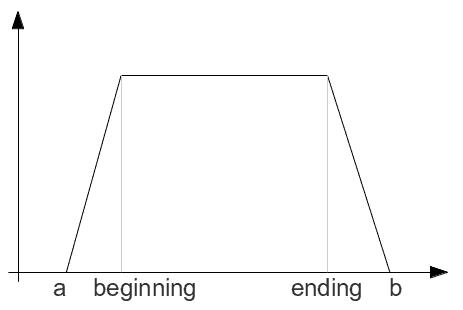
\includegraphics[scale=0.5]{Fig4}
\par\end{centering}

\protect\caption{\label{fig:Trapezium}A Trapezium}
\end{figure}


Next step is to present relation formulas for approaching Trapezium
relation handling. As pointed out before, the sufficient means for
having the relation formulas being handled by the generic mechanism
provided in the previous section is to define calculations for \emph{before},
\emph{same} and \emph{after}. Next couple of sections have been dedicated
to this subject, with an intended emphasis on the Trapezium model.


\subsection{\label{sub:Convolution}Convolution Logic}

Convolution is perhaps the best-suited way to approach studying the
relations between two events in a pure probabilistic context. Assuming
the two random variables X and Y belong, respectively, to the probability
measures \emph{F} and \emph{G} in the $\left(R,~+\right)$ space,
$Convolve\left(F,~-G\right)$ yields the probability distribution
for the random variable $X-Y$ (\emph{-G} denotes \emph{G} horizontally
inversed). Knowing the distribution of $X-Y$ variable is of importance
since the amount that the two measures overlap, or more precisely,
are \emph{same}, before and \emph{after}, could be calculated from
it:
\begin{enumerate}
\item $a{}_{F}<X<b_{F}$
\item $a{}_{G}<Y<b_{G}$
\item $\left(1,~2\right)\Rightarrow$$a{}_{F}-a{}_{G}<X-Y<b_{F}-b_{G}$,
we transform $Convolve\left(F,~-G\right)$ function to fall within
this interval
\item let $a_{H}=max\left(a{}_{F},~a{}_{G}\right)$ and $b_{H}=min\left(b{}_{F},~b{}_{G}\right)$
\item overlap interval of $F$ and $G$ is $\left[a{}_{H},~b{}_{H}\right]$
\emph{iff} $a{}_{H}<b{}_{H}$, these are the bounds in which \emph{F}
and \emph{G} could be the \emph{same}
\item let $L=\left|a_{H}-b_{H}\right|$
\item $before\left(F,~G\right)=\intop_{-\infty}^{-L}Convolve\left(F,~-G\right)dt$
\item $same\left(F,~G\right)=\intop_{-L}^{L}Convolve\left(F,~-G\right)dt$
\item $after\left(F,~G\right)=\intop_{L}^{+\infty}Convolve\left(F,~-G\right)dt$
\end{enumerate}
One catch in the above approach is that not all distributions have
finite start and end bounds, normal for example, falls is $\left(-\infty,~+\infty\right)$.
This could be dealt with by the \emph{Interval} operation that all
standard distributions support. $Interval\left(dist,~\alpha\right)$
calculates the bounds that cover $\alpha$ portion of the distribution.
Setting $\alpha=1-\varepsilon$ guarantees getting finite bounds for
any distribution.

Fig \ref{fig:Convolution-Examples} shows the outcome of the convolution
logic for a number of distributions, while Fig \ref{fig:Convolution-Interpolation}
demonstrates how \emph{before}, \emph{same} and \emph{after} interpolate
by having \emph{G} fixed in the center and sliding \emph{F} from left
to right.

\begin{figure}
\protect\caption{\label{fig:Convolution-Examples}Convolution Logic Examples}
\end{figure}


\begin{figure}
\protect\caption{\label{fig:Convolution-Interpolation}Interpolation of \emph{same},
\emph{before} and \emph{after} in Convolution Logic}
\end{figure}



\subsection{\label{sub:Geometric-Mean}Geometric Mean Logic}

A desired feature for fuzzy degrees corresponding to relations is
for them to vary linearly, this feature is missing in the Convolution
Logic as evident in Fig \ref{fig:Convolution-Interpolation}. Consequently,
the need for a logic that qualifies in this context seems obvious.
A simple, yet effective measure is Geometric Mean (\emph{GM}). \emph{GM}
has a subtle quality, it amounts to zero when either of the operands
are zero. Thus, it provides a solid ground for defining \emph{same:}
\begin{enumerate}
\item let \emph{F and G} be probability measures
\item $H\left(t\right)=\sqrt{F\left(t\right)G\left(t\right)},~t\in\left(-\infty,~+\infty\right)$
\item $same\left(F,~G\right)=\int_{-\infty}^{+\infty}H\left(t\right)dt$
\end{enumerate}
In addition, we would like \emph{before} and \emph{after} to interpolate
linearly in a sensible manner, partitioning the $1-same$ space, we
will utilise four standard attributes of probability distributions,
mean ($\mu$), standard deviation ($\sigma$), skewness (\emph{s})
and kurtosis (\emph{k}):
\begin{enumerate}
\item $F^{\prime}\left(t\right)=F\left(\sigma_{F}t+\mu_{F}\right)$ and
$G^{\prime}\left(t\right)=G\left(\sigma_{G}t+\mu_{G}\right)$, $F^{\prime}$
and $G^{\prime}$ are standardised versions of \emph{F} and \emph{G}
\item $H^{\prime}\left(t\right)=$$\sqrt{F^{\prime}\left(t\right)G^{\prime}\left(t\right)}$
\item $\alpha=\left|\sigma_{F}-\sigma_{G}\right|+\left|s_{F}-s_{G}\right|+\left|k_{F}-k_{G}\right|$
\item $H^{\prime\prime}\left(t\right)=H^{\prime}\left(\frac{t}{\alpha}\right)$
\item $\delta=\mu_{F}-\mu_{G}$
\item $before\left(F,~G\right)=$$\frac{\intop_{\delta}^{+\infty}H^{\prime\prime}\left(t\right)dt}{\intop_{-\infty}^{+\infty}H^{\prime\prime}\left(t\right)dt}$
\item $after\left(F,~G\right)=$$\frac{\intop_{-\infty}^{\delta}H^{\prime\prime}\left(t\right)dt}{\intop_{-\infty}^{+\infty}H^{\prime\prime}\left(t\right)dt}$
\end{enumerate}

\section{\label{sec:Composition}Probabilistic Estimation of a Fuzzy Interval
Relation Composition Table}

Keyvan will explain the approach to generating a composition table
probabilistically

A graph illustrating the transitivity of precedence rule should be
presented, because 3D graphs are pretty and shiny

We can give example results on the precedence rule, and leave full
discussion of the composition table till later..

\bibliography{allen}
 \bibliographystyle{plain}

% that's all folks

\end{document}
